\subsection{Helioviewer}\label{ssec:hv}

SunPy provides the ability to download images hosted by the
Helioviewer Project (\url{http://helioviewer.org}).  
The aim of the Helioviewer Project is to enable
the exploration of solar and heliospheric data from multiple data
sources (such as instrumentation and feature/event catalogues) via
easy-to-use visual interfaces.  The primary data provided by the
Helioviewer Project are images in the JPEG2000 format (for further
details on the Helioviewer Project see \cite{muller2009}). The
JPEG2000 files are typically highly compressed compared to the source
FITS files they are generated from, and so can be a used as a shortcut
to visualise large amounts of data from multiple sources.  SunPy is
also used in Helioviewer production servers to manage the download and
ingestion of JPEG2000 files from remote servers.

The Helioviewer Project categorises image data based on the physical
construction of the source instrument, using a simple hierarchy:
observatory $\rightarrow$ instrument $\rightarrow$ detector
$\rightarrow$ measurement, where '$\rightarrow$' means 'provides
(possibly multiple)'.  Each Helioviewer Project JPEG2000 file contains
metadata which are based (in part) on the original FITS header
information, and carry sufficient information to permit overlay with
other Helioviewer JPEG2000 files. Images can be accessed either as
PNGs (Section \ref{sssec:hv:png}) or as JPEG2000 files (Section
\ref{sssec:hv:jp}).

\subsubsection{Download a PNG file}\label{sssec:hv:png}


Listing \ref{code:hv:downloadlatestpng} demonstrates how to download a
PNG image of the latest AIA 304$\,$\AA\ image available on
\url{Helioviewer.org}.

\begin{listing}[H]
\begin{minted}[bgcolor=bg]{pycon}
>>> from sunpy.net.helioviewer import HelioviewerClient
>>> hv = HelioviewerClient()
>>> hv.download_png('2099/01/01', 4.8, "[SDO,AIA,AIA,304,1,100]",
...                 x0=0, y0=0, width=512, height=512)
\end{minted}
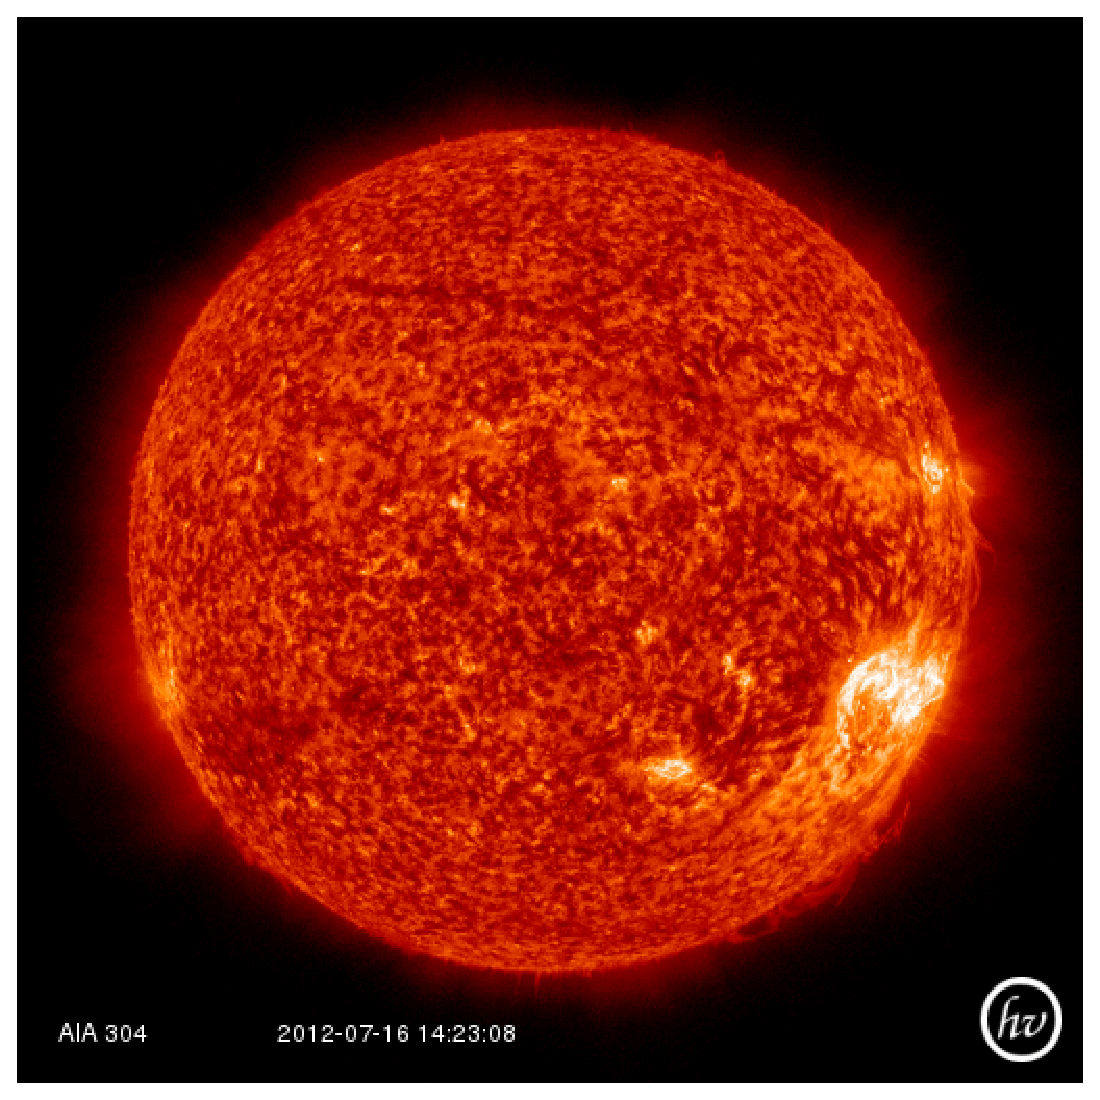
\includegraphics[width=0.8\columnwidth]{helioviewer_latest_aia_304}
%centered image?
\caption{Acquisition of a PNG file showing the latest AIA 304\AA\ image 
available at \url{www.helioviewer.org}.}
\label{code:hv:downloadlatestpng}
\end{listing}

The first argument is the requested time of the image.  Helioviewer
selects images closest to the requested time.  In this case, the
requested time is in the future and so Helioviewer will find the most
recent available image.  The second argument refers to the image
resolution in arcseconds per pixel (larger values mean lower
resolution).  The third argument is a comma-delimited string detailing
the requested observatory $\rightarrow$ instrument $\rightarrow$
detector $\rightarrow$ measurement combination.  The final two numbers
in this string are the visibility and the opacity of the this image
layer (1/0 is visible/invisible with opacity in the range
$0\rightarrow100$, with $100$ meaning fully opaque).  The quantities
$x0$ and $y0$ are the $x$ and $y$ centre points about which to centre
the image (measured in helio-projective cartesian co-ordinates) and
the \texttt{width} and \texttt{height} are the pixel values for the
image dimensions.

It should be noted that the filename of the returned file has the date
and time of the requested time, which is not the time of the
observation shown in the PNG image.  This is because of the
Helioviewer API.  The API request finds images closest to the
requested time. But since the user may ask for images from multiple
sources, and each of them may have a different observation time, it is
unclear which time is the most appropriate to associate with the
resultant image.  The Helioviewer API does not select between any of
the image observation times, but instead returns an image filename
based on the request time, resulting in predictable filenames.

The Helioviewer API allows composition and overlay of images from
multiple sources, based on the positioning metadata in the source FITS
file.  SunPy accesses this overlay/composition capability through the
\texttt{download\_png} method of the Helioviewer client.  Listing
\ref{code:hv:overlaid} gives an example of the composition of three
separate images in to a single image.

\begin{listing}[H]
\begin{minted}[bgcolor=bg]{pycon}
>>> hv.download_png('2099/01/01', 6,
...                 "[SDO,AIA,AIA,304,1,100],[SDO,AIA,AIA,193,1,50]"+
...                 "[SOHO,LASCO,C2,white-light,1,100]",
...                 x0=0, y0=0, width=768, height=768)
\end{minted}
\begin{center}
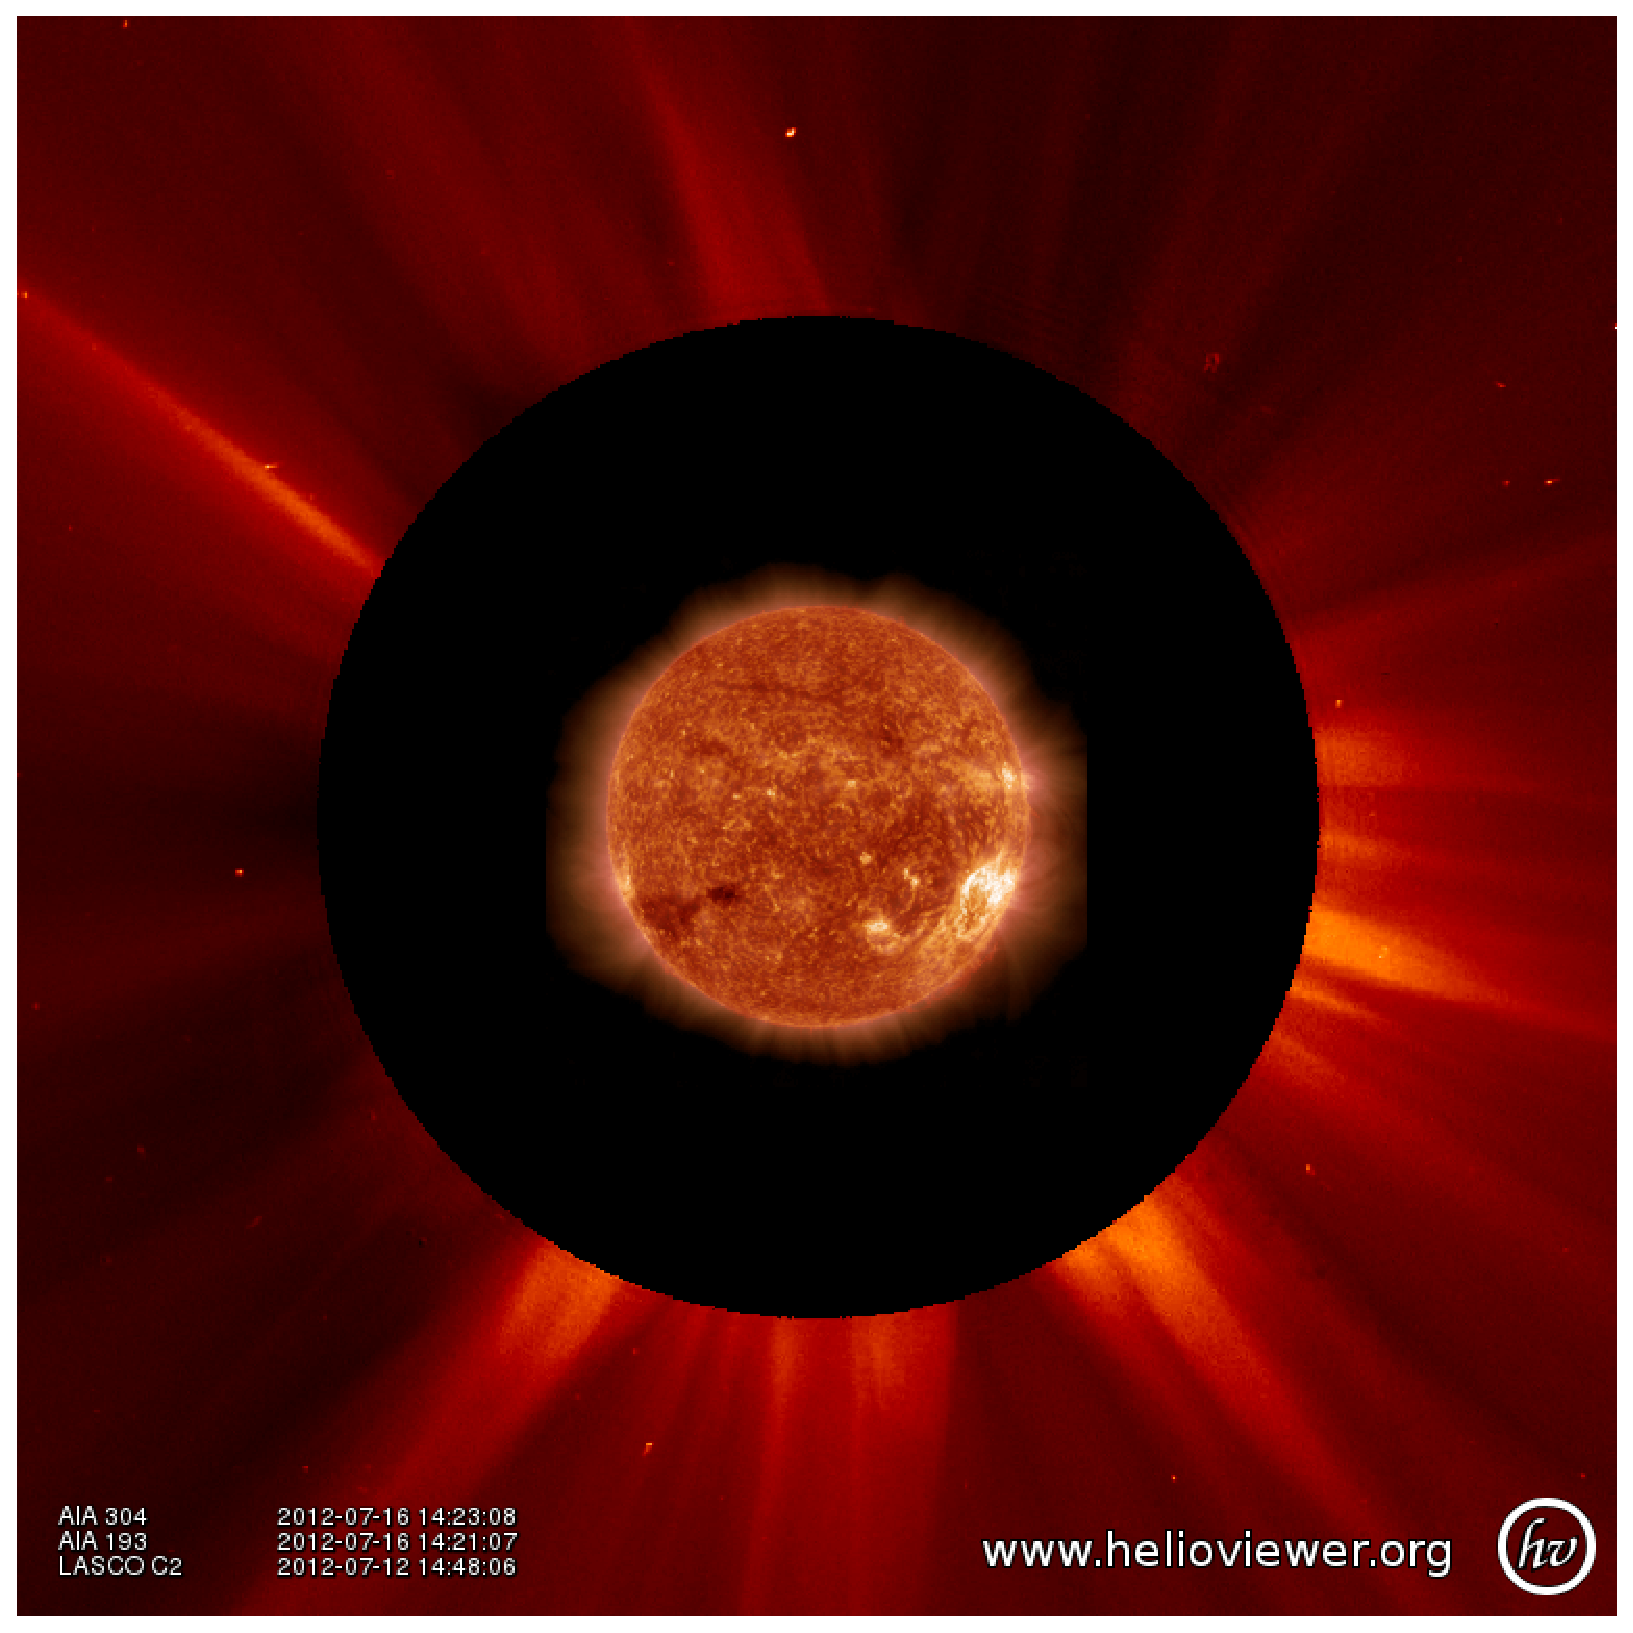
\includegraphics[width=0.8\columnwidth]{helioviewer_overlay_example}
\end{center}
\caption{Acquisition of a PNG image composed from data from three
  separate sources.}
\label{code:hv:overlaid}
\end{listing}

The principle difference between Listings~\ref{code:hv:overlaid} and 
\ref{code:hv:downloadlatestpng} is in the layer string (the third
argument).  The layer string has three separate comma separated
entries detailing the data source, its visibility and its opacity.
This functionality makes it simple for SunPy users to generate complex
images from multiple, correctly overlaid, image data sources.

\subsubsection{Download a JPEG2000 file}\label{sssec:hv:jp}


As noted above, Helioviewer JPEG2000 files contain metadata that allow
positioning of the image data.  There is sufficient metadata in each
file to permit the creation of a SunPy map object (see Section
\ref{ssec:map}) from a Helioviewer JPEG2000 file.  This allows image
data to be manipulated in the same way as any other map object.

Reading JPEG2000 file into a SunPy session requires installing two
other pieces of software. The first, \texttt{OpenJPEG}, is an open
source library for reading and writing JPEG2000 files
(\url{http://www.openjpeg.org}).  The other package required is
\texttt{glymur}, (\url{https://github.com/quintusdias/glymur}), an
interface between Python and the OpenJPEG libraries (note that these
packages are {\it not} required to use the functionality described in
Section \ref{sssec:hv:png}).

Listing \ref{code:downloadjp2} demonstrates the querying, downloading,
reading and conversion of a Helioviewer JPEG2000 file into a SunPy Map
object.  This functionality allows users to visualise and manipulate
Helioviewer-supplied image data in an identical fashion to a SunPy map
object generated from FITS data (see Section \ref{sec:map}).

\begin{listing}[H]
\begin{minted}[bgcolor=bg]{pycon}
>>> filepath = hv.download_jp2('2012/07/05 00:30:00',
...                            observatory='SDO',
...                            instrument='HMI', detector='HMI', 
...                            measurement='continuum')
>>> from sunpy.map import Map
>>> Map(filepath).submap([200,550],[-400,-200]).peek()
\end{minted}
\begin{center}
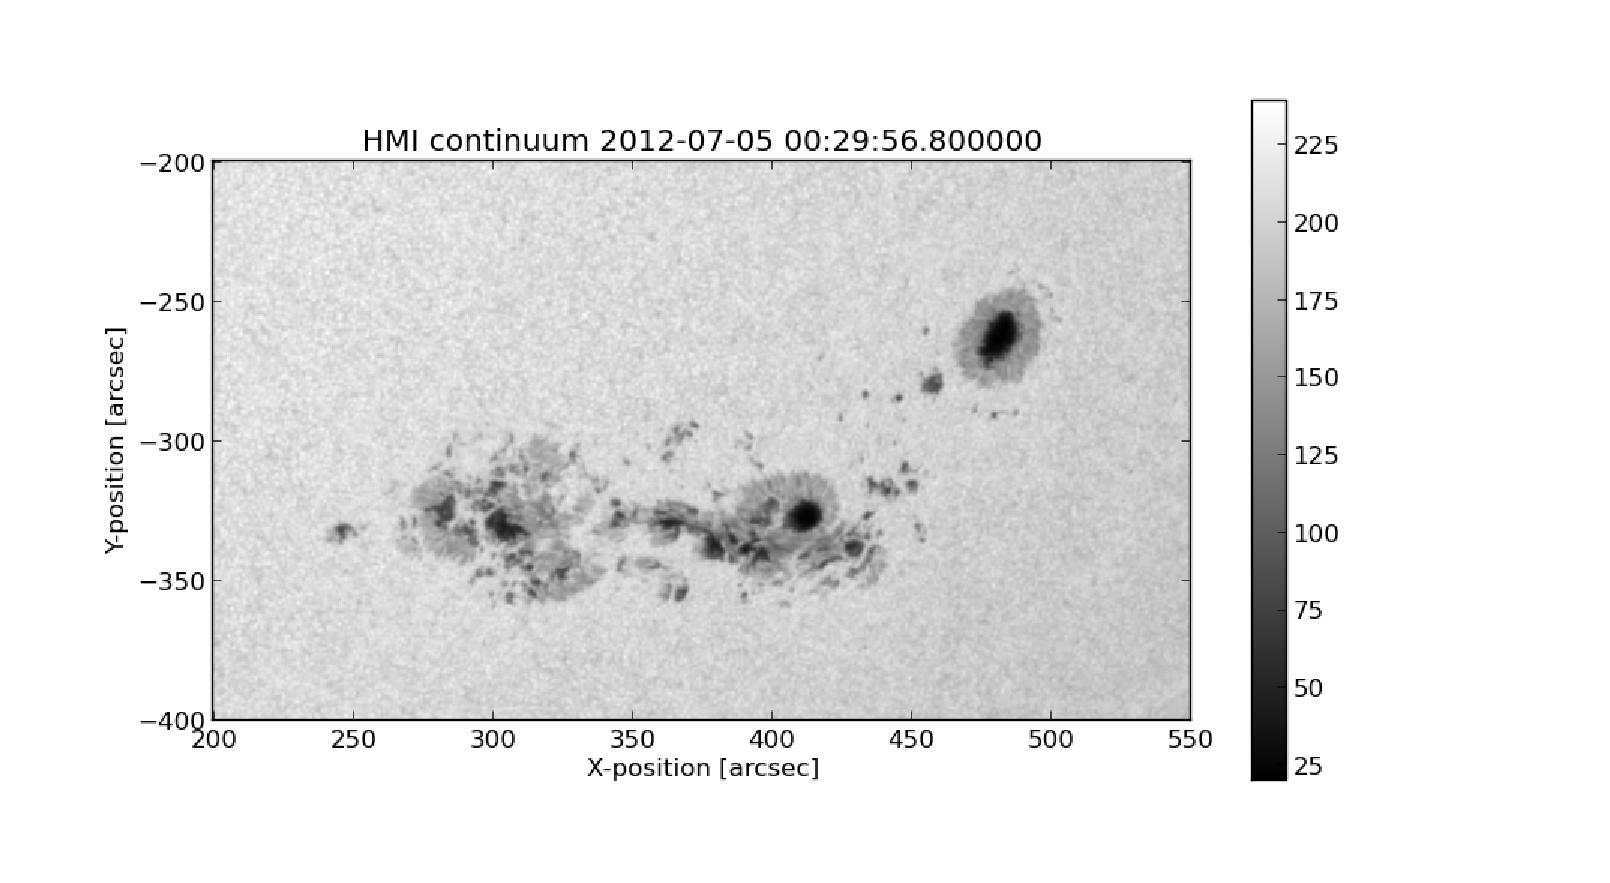
\includegraphics[width=0.8\columnwidth]{helioviewer_hmi_continuum_jp2_to_map}
\end{center}
\caption{Acquisition and display of a Helioviewer JPEG2000 file as a
  SunPy map object.}
\label{code:downloadjp2}
\end{listing}
